\section{Auswertung}
\subsection{Einfachspalt}
Es soll die Spaltbreite ermittelt werden, indem die Aperturfunktion der Blende
auf das Beugungsbild zurückgeführt wird. Das Intensitätsmuster des Beugungsbildes
wurde punktweise aufgenommen, die Messwerte dazu befinden sich in \autoref{tab:10}.
Die Ausgleichsfunktion nach \autoref{eqn:11} ist \autoref{abb:10} zu entnehmen.
\begin{equation}
    \label{eqn:11}
    I\left(\Phi\right) = A^2 \cdot \text{sinc}^2\left(b \cdot \Phi\right) 
\end{equation}
\noindent Durch die Ausgleichsrechnung ergeben sich folgende Parameter:
\begin{align}
    \text{A} = & \qty{0.7156(0.0015)}{\micro\ampere} \\
    \text{b} = & \qty{216.03(0.94)}{\micro\meter}
\end{align}
Dabei gibt der Parameter $b$ die Breite des Spaltes an an dem das Licht gebeugt
wurde. Somit beträgt die experimentell ermittelte breite des Spaltes 
$\qty{0.216(0.0094)}{\milli\meter}$.

\begin{table}[H]
    \centering
    \caption{Messwerte der Intensitätsverteilung des Einzelspalts.}
    \label{tab:10}
    \begin{tblr}{
        colspec = {S S S S S S},
        row{1} = {guard, mode=math},
      }
    \toprule
    \text{x}/ \unit{\milli\meter} & \text{I}/ \unit{\micro\ampere} &
    \text{x}/ \unit{\milli\meter} & \text{I}/ \unit{\micro\ampere} & 
    \text{x}/ \unit{\milli\meter} & \text{I}/ \unit{\micro\ampere} \\
    \midrule
    -25   & 0.002  & -7   & 0.012 & 4   & 0.060 \\
    -24   & 0.002  & -6.5 & 0.008 & 4.5 & 0.040 \\
    -23   & 0.000  & -6   & 0.006 & 5   & 0.014 \\
    -22   & 0.000  & -5.5 & 0.010 & 5.5 & 0.006 \\
    -21   & 0.002  & -5   & 0.020 & 6   & 0.004 \\
    -20   & 0.002  & -4.5 & 0.040 & 6.5 & 0.008 \\
    -19   & 0.002  & -4   & 0.090 & 7   & 0.014 \\
    -18   & 0.000  & -3.5 & 0.140 & 7.5 & 0.018 \\
    -17   & 0.000  & -3   & 0.200 & 8   & 0.020 \\
    -16   & 0.002  & -2.5 & 0.280 & 8.5 & 0.018 \\
    -15   & 0.004  & -2   & 0.340 & 9   & 0.016 \\
    -14   & 0.006  & -1.5 & 0.420 & 9.5 & 0.012 \\
    -13   & 0.006  & -1   & 0.460 & 10  & 0.008 \\
    -12   & 0.004  & -0.5 & 0.500 & 11  & 0.002 \\
    -11   & 0.002  & 0    & 0.520 & 12  & 0.004 \\
    -10.5 & 0.004  & 0.5  & 0.500 & 13  & 0.006 \\
    -10   & 0.006  & 1    & 0.460 & 14  & 0.006 \\
    -9.5  & 0.010  & 1.5  & 0.400 & 15  & 0.004 \\
    -9    & 0.014  & 2    & 0.340 & 16  & 0.002 \\
    -8.5  & 0.016  & 2.5  & 0.260 & 17  & 0.002 \\
    -8    & 0.017  & 3    & 0.200 & 18  & 0.004 \\
    -7.5  & 0.016  & 3.5  & 0.120 & 19  & 0.004 \\
    \bottomrule 
    \end{tblr}
\end{table}
\noindent Jegliche Stromwerte sind mit einem relativen Fehler von $\pm 0.002
\, \unit{\micro\ampere}$ behaftet.

\label{sec:Auswertung}
\begin{figure}[H]    
    \centering
    \caption{Ausgleichsrechnung zur Intensitätsverteilung des Einfachspaltes.}
    \label{abb:10}
    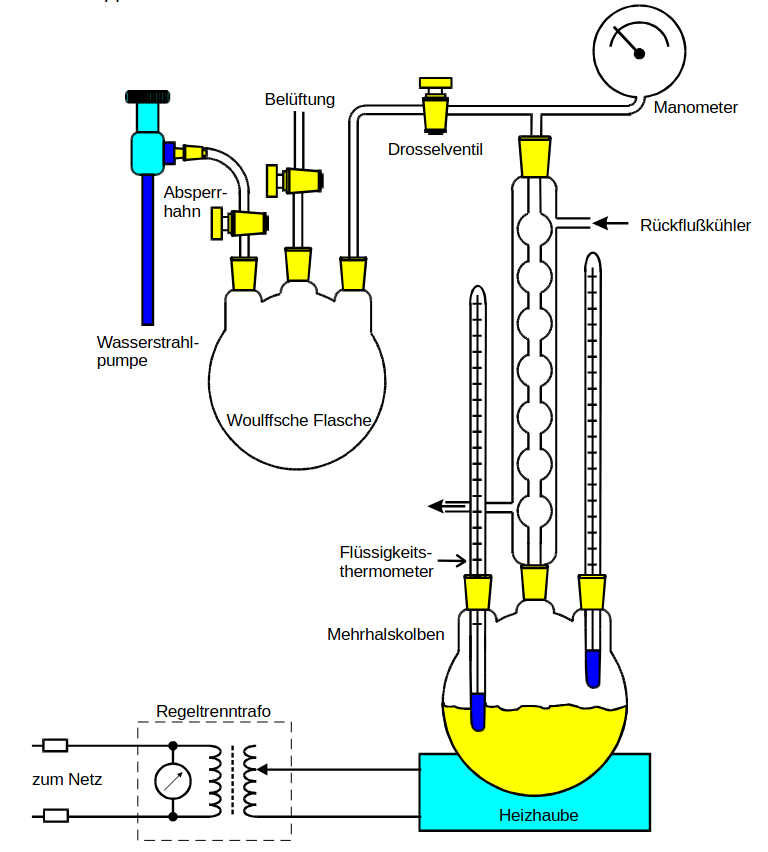
\includegraphics{teil1.pdf}
\end{figure}





\subsection{Doppelspalt}
Ein ähnliches Vorgehen wird bei der Bestimmung der Breite des Doppelspaltes
angewendet. Allerdings wird eine etwas andere Funktion für die Ausgleichsrechnung
verwendet. Diese befindet sich in \autoref{eqn:10}.
\begin{equation}
    \label{eqn:10}
    I\left(\Phi\right) = A^2 \cdot \text{sinc}^2\left(b \cdot \left(x - d\right)\right)  \cdot \cos^2{\left(c \cdot \left(x - d\right)\right)}
\end{equation}
\noindent Die Messdaten der Messung am Doppelspalt befinden sich in \autoref{tab:11}
Die dazugehörige Ausgleichsrechnung ist in \autoref{abb:11} visualisiert.
Die Ausgleichsrechnung durch einen curve Fit des python Paketes scipy ergibt
die Parameter:
\begin{align}
    \text{A} = & \qty{0.6249(0.0078)}{\micro\ampere} \\
    \text{b} = & \qty{121.601(3.079)}{\micro\meter}\\
    \text{c} = & \qty{2809(8)}{} \\
    \text{d} = & \qty{-0.0002(0)}{\milli\meter}
\end{align}
\noindent Daraus ergibt sich für die experimentellen Spaltbreiten des Doppelspalts:
\begin{equation}
    b_\text{Doppelspalt} = \qty{0.12(0.30)}{\milli\meter}.
\end{equation}
\noindent
% \begin{table}[H]
%     \centering
%     \caption{Messwerte der Intensitätsverteilung des Doppelspalts.}
%     \label{tab:11}
%     \begin{tblr}{
%         colspec = {S S | S S | S S | S S},
%         row{1} = {guard, mode=math},}
%            \toprule
%             \text{x}/ \unit{\milli\meter} & \text{I}/ \unit{\micro\ampere}& \text{x} /\unit{\milli\meter} & \text{I} /\unit{\micro\ampere}& \text{x} /\unit{\milli\meter} & \text{I} /\unit{\micro\ampere} & \text{x} /\unit{\milli\meter} & \text{I}/ \unit{\micro\ampere}\\
%            \midrule
%            -25   & 0.003 & +-0.001 & -8.5  & 0.018 & +-0.001 &      0.5    & 0.020   +-0.01     &    9.5    & 0.004    +-0.001   \\              
%            -24.5 & 0.002 & +-0.001 & -8.25 & 0.014 & +-0.001 &      0.75   & 0.100   +-0.01     &    9.75   & 0.002    +-0.001   \\    
%            -24   & 0.001 & +-0.001 & -8    & 0.004 & +-0.001 &      1      & 0.300   +-0.01     &    10     & 0.002    +-0.001   \\    
%            -23.5 & 0.003 & +-0.001 & -7.75 & 0.010 & +-0.001 &      1.25   & 0.400   +-0.01     &    10.5   & 0.004    +-0.001   \\    
%            -23   & 0.000 & +-0.001 & -7.5  & 0.030 & +-0.001 &      1.5    & 0.240   +-0.01     &    11     & 0.008    +-0.001   \\    
%            -22.5 & 0.001 & +-0.001 & -7.25 & 0.056 & +-0.001 &      1.75   & 0.060   +-0.01     &    11.5   & 0.004    +-0.001   \\    
%            -22   & 0.002 & +-0.001 & -7    & 0.050 & +-0.001 &      2      & 0.040   +-0.01     &    12     & 0.004    +-0.001   \\    
%            -21.5 & 0.001 & +-0.001 & -6.75 & 0.020 & +-0.001 &      2.25   & 0.200   +-0.01     &    12.5   & 0.012    +-0.001   \\    
%            -21   & 0.002 & +-0.001 & -6.5  & 0.006 & +-0.001 &      2.5    & 0.300   +-0.01     &    13     & 0.004    +-0.001   \\
%            -20.5 & 0.003 & +-0.001 & -6.25 & 0.040 & +-0.001 &      2.75   & 0.280   +-0.01     &    13.5   & 0.006    +-0.001   \\
%            -20   & 0.002 & +-0.001 & -6    & 0.100 & +-0.001 &      3      & 0.140   +-0.01     &    14     & 0.012    +-0.001   \\
%            -19.5 & 0.002 & +-0.001 & -5.75 & 0.140 & +- 0.01 &      3.25   & 0.020   +-0.01     &    14.5   & 0.002    +-0.001   \\
%            -19   & 0.001 & +-0.001 & -5.5  & 0.100 & +- 0.01 &      3.5    & 0.040   +-0.01     &    15     & 0.006    +-0.001   \\
%            -18.5 & 0.001 & +-0.001 & -5.25 & 0.020 & +- 0.01 &      3.75   & 0.140   +-0.01     &    15.5   & 0.002    +-0.001   \\    
%            -18   & 0.002 & +-0.001 & -5    & 0.020 & +- 0.01 &      4      & 0.222   +-0.01     &    16     & 0.003    +-0.001   \\
%            -17.5 & 0.001 & +-0.001 & -4.75 & 0.120 & +- 0.01 &      4.25   & 0.140   +-0.01     &    16.5   & 0.001    +-0.001   \\
%            -17   & 0.000 & +-0.001 & -4.5  & 0.220 & +- 0.01 &      4.5    & 0.040   +-0.01     &    17     & 0.002    +-0.001   \\
%            -16.5 & 0.002 & +-0.001 & -4.25 & 0.200 & +- 0.01 &      4.75   & 0.000   +-0.01     &    17.5   & 0.003    +-0.001   \\
%            -16   & 0.006 & +-0.001 & -4    & 0.100 & +- 0.01 &      5      & 0.040   +-0.01     &    18     & 0.003    +-0.001   \\    
%            -15.5 & 0.006 & +-0.001 & -3.75 & 0.020 & +- 0.01 &      5.25   & 0.100   +-0.01     &    18.5   & 0.003    +-0.001   \\    
%            -15   & 0.002 & +-0.001 & -3.5  & 0.060 & +- 0.01 &      5.5    & 0.100   +-0.01     &    19     & 0.003    +-0.001   \\    
%            -14.5 & 0.012 & +-0.001 & -3.25 & 0.240 & +- 0.01 &      5.75   & 0.060   +-0.01     &    19.5   & 0.003    +-0.001   \\
%            -14   & 0.006 & +-0.001 & -3    & 0.320 & +- 0.01 &      6      & 0.020   +-0.001    &    20     & 0.003    +-0.001   \\
%            -13.5 & 0.002 & +-0.001 & -2.75 & 0.200 & +- 0.01 &      6.25   & 0.000   +-0.001    &    20.5   & 0.003    +-0.001  \\
%            -13   & 0.012 & +-0.001 & -2.5  & 0.060 & +- 0.01 &      6.5    & 0.040   +-0.001    &    21     & 0.002    +-0.001  \\
%            -12.5 & 0.004 & +-0.001 & -2.25 & 0.020 & +- 0.01 &      6.75   & 0.060   +-0.001    &    21.5   & 0.003    +-0.001  \\
%            -12   & 0.004 & +-0.001 & -2    & 0.140 & +- 0.01 &      7      & 0.040   +-0.001    &    22     & 0.002    +-0.001  \\
%            -11.5 & 0.006 & +-0.001 & -1.75 & 0.400 & +- 0.01 &      7.25   & 0.020   +-0.001    &    22.5   & 0.002    +-0.001  \\
%            -11   & 0.002 & +-0.001 & -1.5  & 0.400 & +- 0.01 &      7.5    & 0.000   +-0.001    &    23     & 0.003    +-0.001  \\
%            -10.5 & 0.002 & +-0.001 & -1.25 & 0.200 & +- 0.01 &      7.75   & 0.000   +-0.001    &    23.5   & 0.002    +-0.001  \\
%            -10   & 0.004 & +-0.001 & -1    & 0.020 & +- 0.01 &      8      & 0.020   +-0.001    &    24     & 0.002    +-0.001  \\
%            -9.75 & 0.004 & +-0.001 & -0.75 & 0.060 & +- 0.01 &      8.25   & 0.020   +-0.001    &    24.5   & 0.003    +-0.001  \\
%            -9.5  & 0.002 & +-0.001 & -0.5  & 0.300 & +- 0.01 &      8.5    & 0.000   +-0.001    &    25     & 0.002    +-0.001  \\
%            -9.25 & 0.002 & +-0.001 & -0.25 & 0.140 & +- 0.01 &      8.75   & 0.000   +-0.001    &       &   \\
%            -9    & 0.004 & +-0.001 & 0     & 0.360 & +- 0.01 &      9      & 0.040   +-0.001    &        &  \\
%            -8.75 & 0.012 & +-0.001 & 0.25  & 0.140 & +- 0.01 &      9.25   & 0.004   +-0.001    &         & \\
%         \bottomrule
%     \end{tblr}
% \end{table}

\begin{table}[H]
    \centering
    \caption{Messwerte der Intensitätsverteilung des Doppelspalts.}
    \label{tab:11}
    \begin{tblr}{
        colspec = {S S S S S S},
        row{1} = {guard, mode=math},
      }
    \toprule
    \text{x}/ \unit{\milli\meter} & \text{I}/ \unit{\micro\ampere} &
    \text{x}/ \unit{\milli\meter} & \text{I}/ \unit{\micro\ampere} & 
    \text{x}/ \unit{\milli\meter} & \text{I}/ \unit{\micro\ampere} \\
    \midrule
    -25   & 0.003 & -8.5  & 0.018 & 0.5  & 0.020 & 9.5  & 0.004 \\
    -24.5 & 0.002 & -8.25 & 0.014 & 0.75 & 0.100 & 9.75 & 0.002 \\
    -24   & 0.001 & -8    & 0.004 & 1    & 0.300 & 10   & 0.002 \\
    -23.5 & 0.003 & -7.75 & 0.010 & 1.25 & 0.400 & 10.5 & 0.004 \\
    -23   & 0.000 & -7.5  & 0.030 & 1.5  & 0.240 & 11   & 0.008 \\
    -22.5 & 0.001 & -7.25 & 0.056 & 1.75 & 0.060 & 11.5 & 0.004 \\
    -22   & 0.002 & -7    & 0.050 & 2    & 0.040 & 12   & 0.004 \\
    -21.5 & 0.001 & -6.75 & 0.020 & 2.25 & 0.200 & 12.5 & 0.012 \\
    -21   & 0.002 & -6.5  & 0.006 & 2.5  & 0.300 & 13   & 0.004 \\
    -20.5 & 0.003 & -6.25 & 0.040 & 2.75 & 0.280 & 13.5 & 0.006 \\
    -20   & 0.002 & -6    & 0.100 & 3    & 0.140 & 14   & 0.012 \\
    -19.5 & 0.002 & -5.75 & 0.140 & 3.25 & 0.020 & 14.5 & 0.002 \\
    -19   & 0.001 & -5.5  & 0.100 & 3.5  & 0.040 & 15   & 0.006 \\
    -18.5 & 0.001 & -5.25 & 0.020 & 3.75 & 0.140 & 15.5 & 0.002 \\
    -18   & 0.002 & -5    & 0.020 & 4    & 0.222 & 16   & 0.003 \\
    -17.5 & 0.001 & -4.75 & 0.120 & 4.25 & 0.140 & 16.5 & 0.001 \\
    -17   & 0.000 & -4.5  & 0.220 & 4.5  & 0.040 & 17   & 0.002 \\
    -16.5 & 0.002 & -4.25 & 0.200 & 4.75 & 0.000 & 17.5 & 0.003 \\
    -16   & 0.006 & -4    & 0.100 & 5    & 0.040 & 18   & 0.003 \\
    -15.5 & 0.006 & -3.75 & 0.020 & 5.25 & 0.100 & 18.5 & 0.003 \\
    -15   & 0.002 & -3.5  & 0.060 & 5.5  & 0.100 & 19   & 0.003 \\
    -14.5 & 0.012 & -3.25 & 0.240 & 5.75 & 0.060 & 19.5 & 0.003 \\
    -14   & 0.006 & -3    & 0.320 & 6    & 0.020 & 20   & 0.003 \\
    -13.5 & 0.002 & -2.75 & 0.200 & 6.25 & 0.000 & 20.5 & 0.003 \\
    -13   & 0.012 & -2.5  & 0.060 & 6.5  & 0.040 & 21   & 0.002 \\
    -12.5 & 0.004 & -2.25 & 0.020 & 6.75 & 0.060 & 21.5 & 0.003 \\
    -12   & 0.004 & -2    & 0.140 & 7    & 0.040 & 22   & 0.002 \\
    -11.5 & 0.006 & -1.75 & 0.400 & 7.25 & 0.020 & 22.5 & 0.002 \\
    -11   & 0.002 & -1.5  & 0.400 & 7.5  & 0.000 & 23   & 0.003 \\
    -10.5 & 0.002 & -1.25 & 0.200 & 7.75 & 0.000 & 23.5 & 0.002 \\
    -10   & 0.004 & -1    & 0.020 & 8    & 0.020 & 24   & 0.002 \\
    -9.75 & 0.004 & -0.75 & 0.060 & 8.25 & 0.020 & 24.5 & 0.003 \\
    -9.5  & 0.002 & -0.5  & 0.300 & 8.5  & 0.000 & 25   & 0.002 \\
    -9.25 & 0.002 & -0.25 & 0.140 & 8.75 & 0.000 &    &   \\
    -9    & 0.004 & 0     & 0.360 & 9    & 0.040 &     &  \\
    -8.75 & 0.012 & 0.25  & 0.140 & 9.25 & 0.004 &      & \\
    \bottomrule 
    \end{tblr}
\end{table}
\noindent Die Stromwerte im Intervall zwischen $-25 - 6 \unit{\milli\meter}$ unterliegen
dem relativen Fehler von $\pm 0.01 \unit{\micro\ampere}$. Jegliche Restwerte im Bereich von
$6 - 25 \unit{\milli\meter}$ hingegen sind mit einem Fehler von $\pm 0.001 \unit{\micro\ampere}$
behaftet.


\begin{figure}[H]
    \centering
    \caption{Ausgleichsrechnung zur Intensitätsverteilung des Doppelspaltes.}
    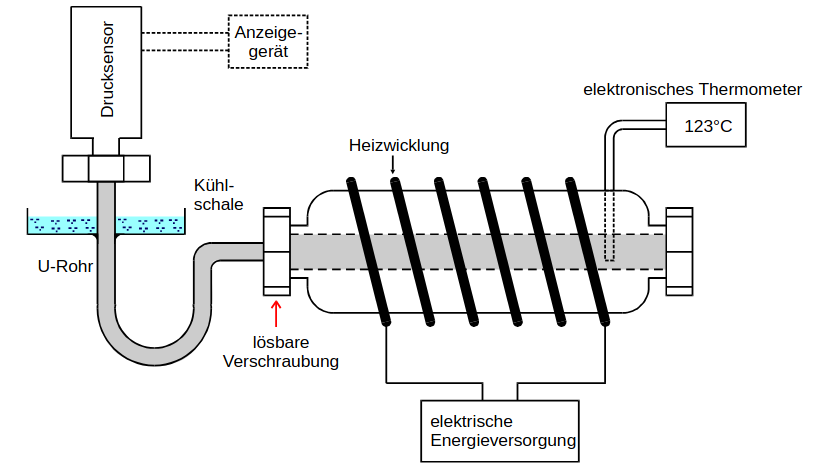
\includegraphics{teil2.pdf}
    \label{abb:11}
\end{figure}

\begin{figure}[H]
    \centering
    \caption{Vergleich der Intensitätsverteilungen Doppelspalt und Einfachspalt.}
    \includegraphics{teil3.pdf}
    \label{abb:12}
\end{figure}


